\documentclass[tikz,border=9pt]{standalone}
\usepackage[T1]{fontenc}\usepackage{lmodern,amsmath,amssymb}
\usetikzlibrary{arrows.meta,positioning,calc}
\begin{document}
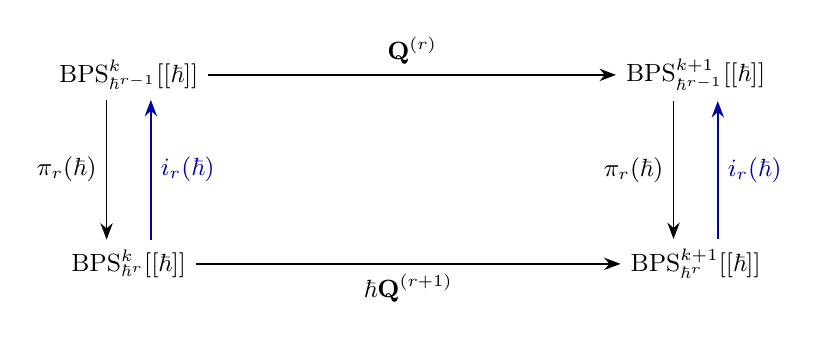
\begin{tikzpicture}[>=Stealth, every node/.style={font=\small},every path/.style={line width=.65pt}]

\node (a) at (-3.6,1.2) {$\mathrm{BPS}_{\hbar^{r-1}}^{k}[[\hbar]]$};
\node (b) at (3.6,1.2) {$\mathrm{BPS}_{\hbar^{r-1}}^{k+1}[[\hbar]]$};
\node (c) at (-3.6,-1.2) {$\mathrm{BPS}_{\hbar^{r}}^{k}[[\hbar]]$};
\node (d) at (3.6,-1.2) {$\mathrm{BPS}_{\hbar^{r}}^{k+1}[[\hbar]]$};
\draw[->] (a) -- node[above] {$\mathbf Q^{(r)}$} (b);
\draw[->] (c) -- node[below] {$\hbar\mathbf Q^{(r+1)}$} (d);
\draw[->] ([xshift=-8pt]a.south) -- node[left] {$\pi_r(\hbar)$} ([xshift=-8pt]c.north);
\draw[->,blue!65!black] ([xshift=8pt]c.north) -- node[right] {$i_r(\hbar)$} ([xshift=8pt]a.south);
\draw[->] ([xshift=-8pt]b.south) -- node[left] {$\pi_r(\hbar)$} ([xshift=-8pt]d.north);
\draw[->,blue!65!black] ([xshift=8pt]d.north) -- node[right] {$i_r(\hbar)$} ([xshift=8pt]b.south);

\end{tikzpicture}
\end{document}
